\chapter{Alkali-doped nanodroplets}

	\lettrine[lines=4,findent=3pt,nindent=0pt]{\color{niceBlue1}I}{n} their 1996 paper\citep{Griffin1996} Griffin and Stringari have argued that almost 100\% Bose-Einstein Condensation could be achieved in the low density surface region of superfluid He at $T=0$, as opposed to only about 10\% in the bulk. It is therefore evident that a minimally perturbing probe capable of investigating the surface of a He cluster is very desirable.

	It was believed\citep{Dalfovo1994} that the alkali atoms reside on the cluster surface. Experimental evidence for this was found\citep{Stienkemeier1995-1,Stienkemeier1995-2,Ancilotto1995} later when it was observed that the laser induced fluoresence (LIF) spectrum of sodium was shifted compared to sodium in the gas phase due to the presence of the He cluster. However, not as much as e.g. rare gas atoms that reside in the interior of the He droplet.
	
	It comes as no surprise then that alkali atoms are a very natural choice for exactly these type of studies.  For example, with a solvation parameter (see Section \ref{sec:helium-droplets}) of $\lambda=0.729$\citep{Anc95}, Rb will remain bound to the surface of the droplet. Furthermore, they have a simple, well known, absorption spectrum. Moreover, their simple, one-valence electron structure allows for detailed theoretical modelling. They introduce only weak perturbations (alkali-helium interaction energies are on the order of 1 cm$^{-1}$\citep{Pat91}). Lastly, theoretical calculations\citep{Ancilotto1995,Kanorsky1994} and experimental spectra\citep{Tabbert1995,Takahashi1993,Beijersbergen1993} of alkali atoms in bulk liquid helium are available for comparison.

	Surprisingly, the study of alkali atoms seeded in highly quantum matrices is relevant to the optimisation of the use of solid hydrogen as a rocket propellant\citep{Carrick1993}.
	
	Given that the alkalis are ideal objects to probe the boundary region of the nanodroplets, the $n\mathrm{p}\,^2\mathrm{P}\!\longleftarrow\!n\mathrm{s}\,^2\mathrm{S}$ transitions of the alkali atoms have attracted much interest from an experimental and theoretical point of view. The spectroscopy of the higher excited states has been thoroughly explored\citep{Log11b,Log11a,Lackner2012,Lackner2013,The11,Fec12,Pif10,Lac11,Theisen2011,Lac13}. The obtained spectra can be successfully reproduced by a pseudo-diatomic model\footnote{Also called the ``frozen droplet'' model. It is equivalent to the DIM model, explained in Section \ref{sec:dim-model}, where the internal degrees of freedom of the droplet are neglected.}, except for the higher excited states, where the model progressively fails due to the limitations imposed by its realm of validity\citep{Sti96,Bunermann2007}. While the the effect of the excited states on the spectra are now fairly well understood, their influence on the following dynamics is largely unexplored.
	
	In this part of the thesis, the results of the real-time dynamics of a single electronically excited rubidium (Rb) atom residing in the surface dimple of a helium nano-droplet are presented. The atom is excited from its ground state 5s$\,^2\Sigma_{1/2}$ to the 5p$\,^2\{\Sigma,\Pi\}$ and 6p$\,^2\{\Sigma,\Pi\}$ manifold. This is a combined experimental and theoretical study.
	
	\section{Experimental setup}

		\begin{figure}[t]
			\begin{center}
				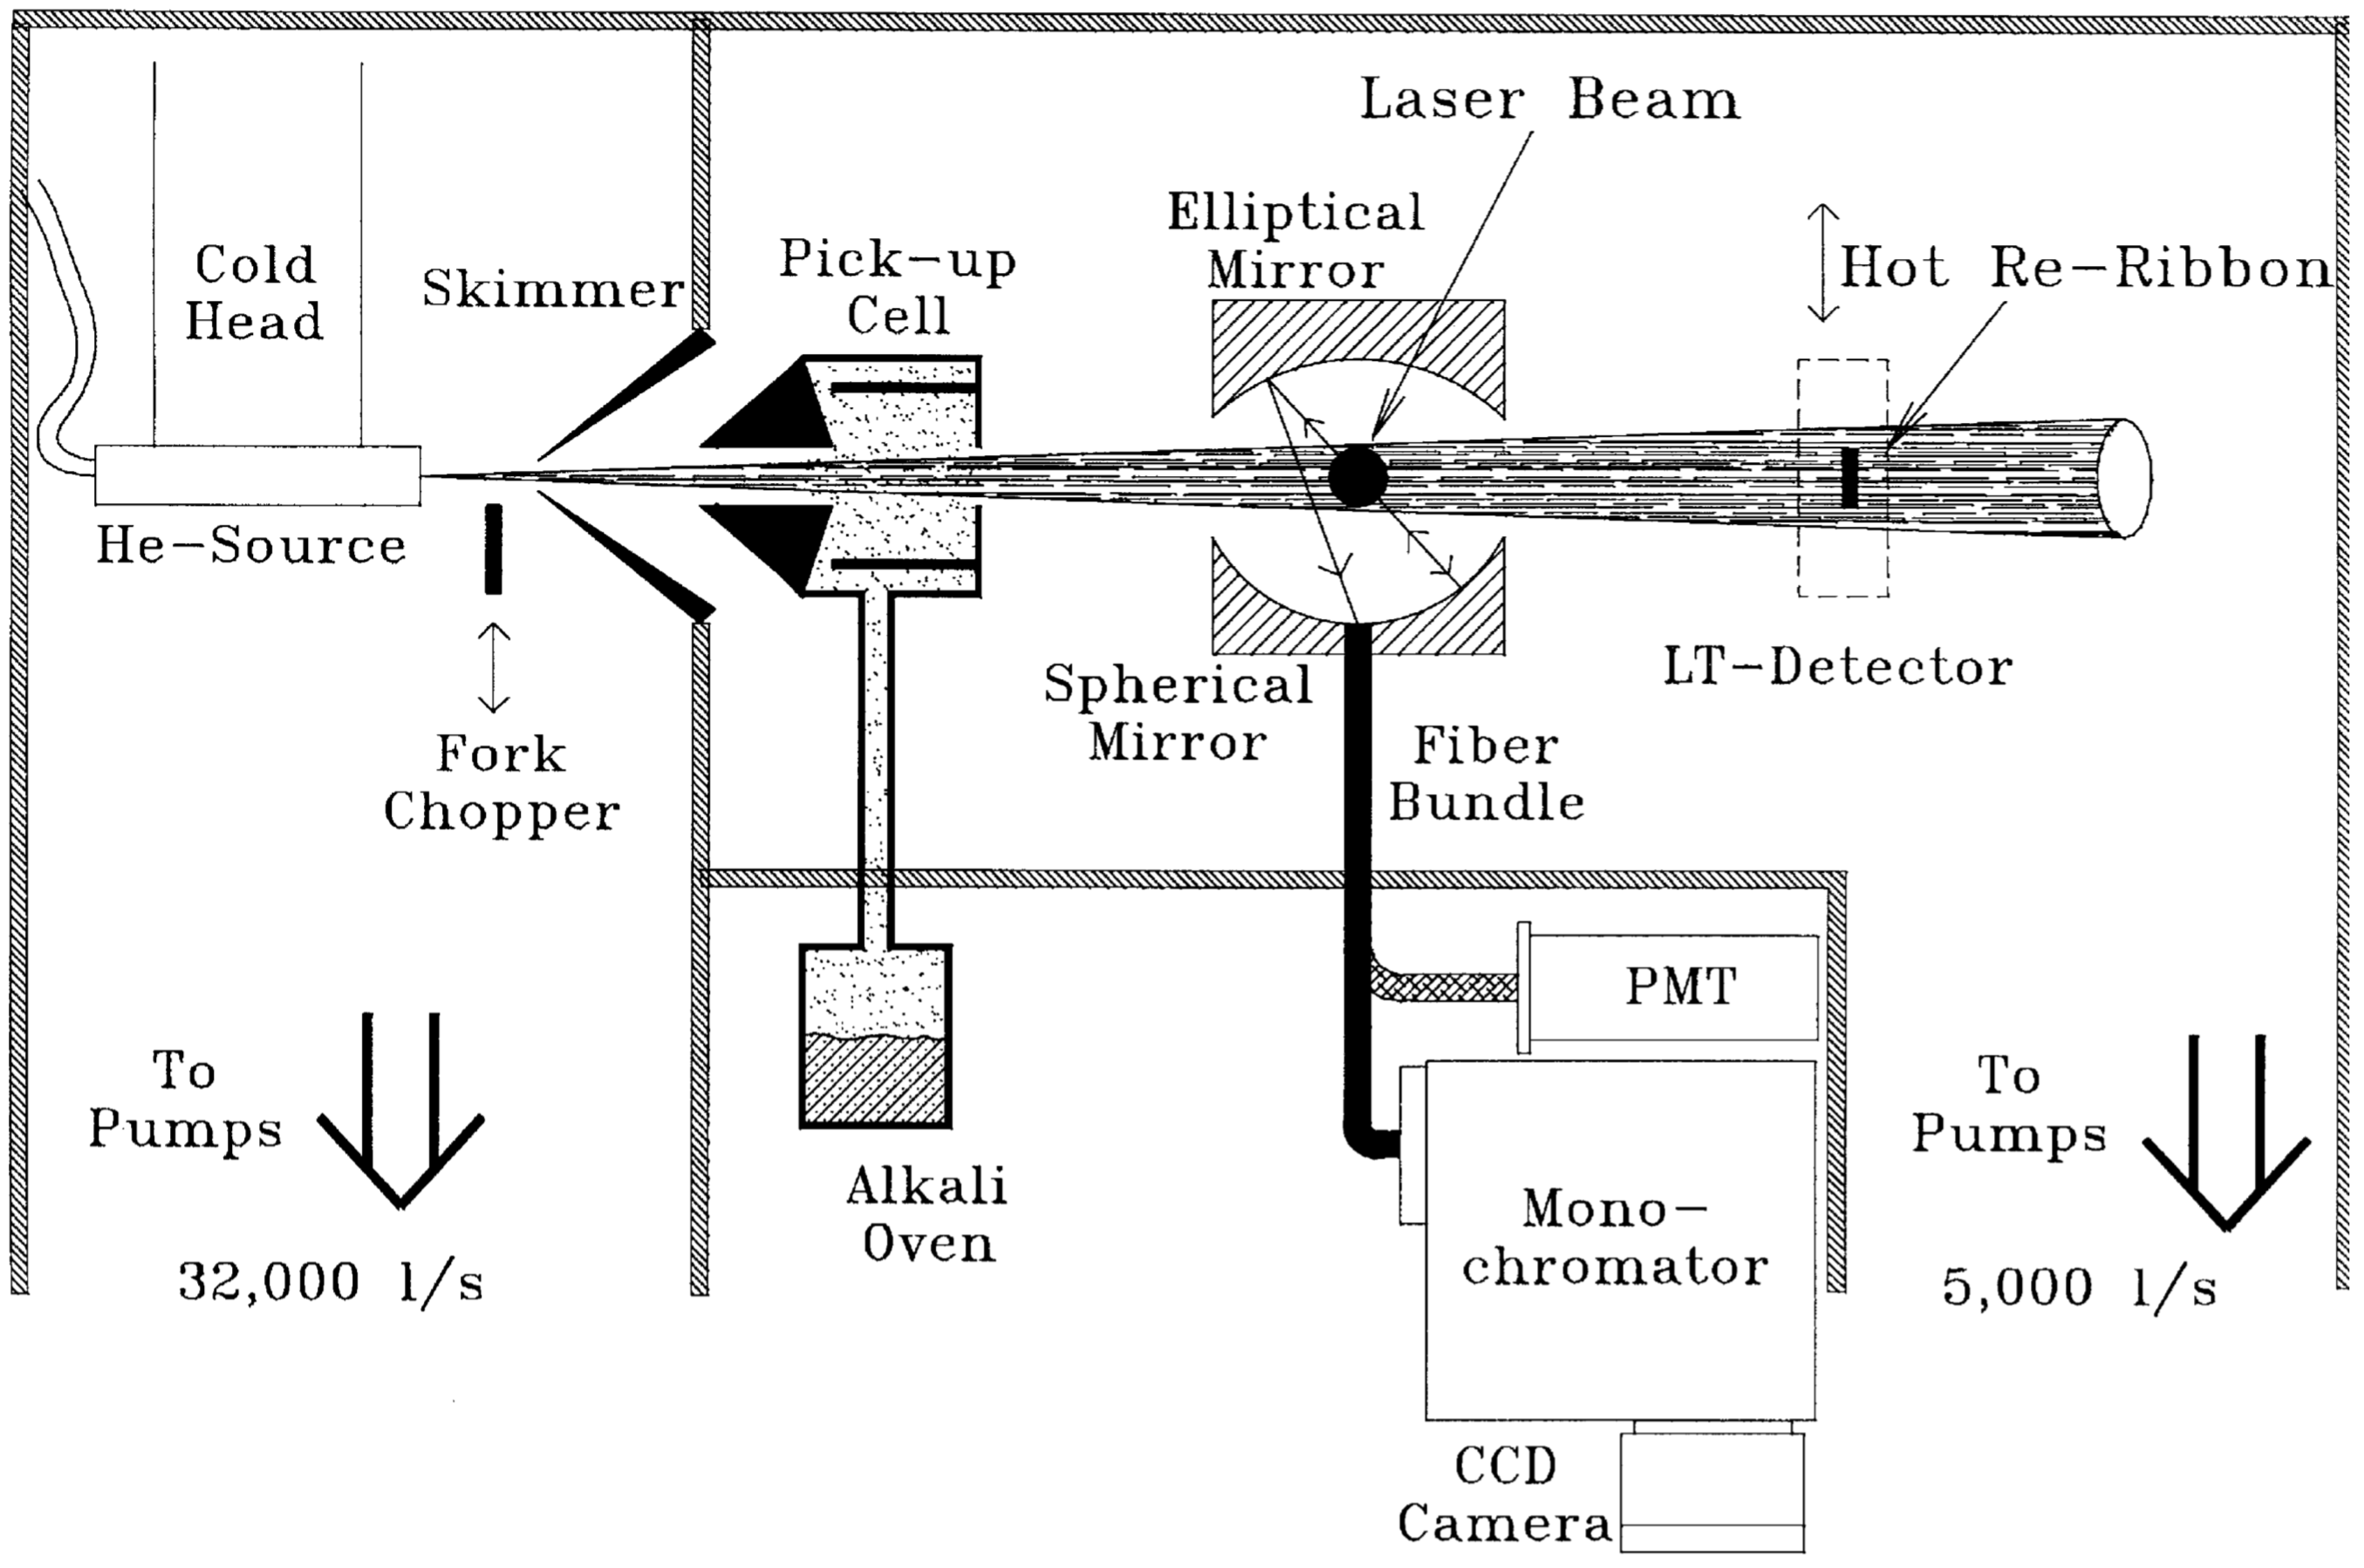
\includegraphics[width=\textwidth]{droplet-beam}
				\caption{Caption}
				\label{fig:droplet-beam}
			\end{center}
		\end{figure}
		
		A beam of large He clusters is produced in a supersonic expansion from a cold nozzle (Fig. \ref{fig:droplet-beam}). The weak He-He binding energy of 7.7 cm$^{-1}$ [22] requires high stagnation pressures and low nozzle temperatures ($T$) for large cluster formation. For a set pressure, nozzle aperture and temperature the droplet sizes are log-normal distributed. Doping of the He clusters realised by sending the beam through a pick-up cell (located a short distance after the skimmer) in which a variable pressure of the alkali is maintained by connecting the pick-up cell with the reservoir through a heated tube. For a chosen average droplet size the average number of dopants picked-up by the droplet is governed by Poissonian statistics and can be controlled with the vapour pressure inside the pickup cell. In their path through the cell the larger clusters pick up alkali atoms without being appreciably deflected. Dissipation of the energy of the captured alkali is likely to occur by evaporation of He atoms from the clusters, the terminal temperature of which rapidly returns to its pre pick-up value ($\sim$0.4 K) [2].
	
		To probe the picked-up alkali atoms a variety of measurement techniques can be employed, e.g. laser induced fluorescence (LIF) spectroscopy, time-resolved pump-probe spectroscopy, photo-electron spectroscopy and velocity map imagining (VMI). The specific ones used in this work will be introduced generally in the next section.%was used. The intersection point of the laser and cluster beam from which the fluorescence photons are collected is located a few centimetres downstream of the pick-up cell. To detect the fluorescence light originating at the point of intersection, the combination of an elliptical and a spherical mirror is used. These two mirrors focus the emitted photons at the entrance of a fibre bundle. Alternatively, a monochromator coupled to a liquid nitrogen cooled CCD detector is used for dispersed fluorescence measurements.